\documentclass[fleqn,10pt]{wlscirep}
\usepackage[utf8]{inputenc}
\usepackage[T1]{fontenc}
\title{Comparing Ordinary Differential Equation and Recurrent Neural Network Modeling of HIV-1 Within-Host Dynamics After Passive Infusion of the Broadly Neutralizing Antibody VRC01}

\author[1,*]{Jonah Hall}
\author[1,*]{Mateusz Faltyn}
\affil[1]{University of British Columbia, Department of Mathematics, Vancouver, V6T 1Z2, Canada}

\affil[*]{these authors contributed equally to this work}

%\keywords{Keyword1, Keyword2, Keyword3}

\begin{abstract}
HIV-1 is a virus that chronically infects over 30 million individuals globally each year and is the cause of the chronic condition of AIDS. In a paper done by Perelson et al, they found that a phagocytosis based logistic clearance model (PLCM) (mediated by antibody dependent cellular phagocytosis (ADCP)) as the dominant mechanism of action best recapitulated the data provided by a publicly available clinical trial done by the NIH in Lynch et al. The PLCM captures the viral dynamics and recapitulates the data well, but one may require a good understanding of mathematics and microbiology as well as the time to isolate the desired results of the model. In a clinical setting, this may not be the most effective manner in which to use the models prediction to make medical assessments. In this paper, we aim to train and evaluate several LSTM-RNN models in the task of predicting HIV viral dynamics using a synthetic dataset generated from running simulations of the PLCM. In comparing four LSTM-RNN models using synthetic data generated from ODE simulation, we found that, to varying degrees of success, these models were able to capture the viral dynamics generated by the system of differential equations.
\end{abstract}
\begin{document}

\flushbottom
\maketitle
% * <john.hammersley@gmail.com> 2015-02-09T12:07:31.197Z:
%
%  Click the title above to edit the author information and abstract
%
\thispagestyle{empty}


%%%%%%%%%%%%%%%%%%%%%%
\section*{Introduction}

HIV-1 is a virus that chronically infects over 30 million individuals globally each year and is the cause of the chronic condition of AIDS. While there is no cure or preventative vaccine (excluding pre-exposure prophylaxis treatments) for this viral infection, antiretroviral therapy (ART) can be used to keep an individual’s viraemia low enough to lead a semi-normal life. Oral intake of one capsule a day is enough to achieve this, however there are certain populations of people (those with mental illness, certain ages and socio-economic status) that are incapable of keeping this treatment regimen. A possible alternative solution comes in the form of broadly neutralizing antibodies (bnAbs). Optimistically, one passive infusion of a bnAb in the blood plasma could keep viremia low for several weeks to months, offering a less intensive treatment regimen. Among the antibodies being evaluated for this purpose are the VRC class of bnAbs isolated by the United States’ National Institute of Health (NIH). One of the more prominent VRC antibodies is VRC$_{01}$, which has undergone several human clinical trials. Several mathematical models have been fitted to the clinical data in order to help explain the viral dynamics and possible mechanisms of action the bnAb uses to combat viral infection. Among the possible mechanisms of action are neutralization (being the most prominent), and a selection or combination of various $F_c$-mediated functions.

In a paper done by Perelson et al,\cite{Cardozo:2021} they found that a phagocytosis based logistic clearance model (PLCM) (mediated by antibody dependent cellular phagocytosis (ADCP)) as the dominant mechanism of action best recapitulated the data provided by a publicly available clinical trial done by the NIH in Lynch et al.\cite{Lynch:2015}

In this model it is assumed that there are two viral populations, one sensitive to the given antibody and one resistant. The parameters $V_s$ and $V_r$ represent the sensitive and resistant viral populations and $I_s$ and $I_r$ the population of infected cells which produces virus at a rate $p$. The viruses are naturally cleared at a rate $c$. The population of target cells is denoted by $T$ and are produced at a rate $\lambda$, and the cells get infected at a rate $\beta V T$. When free virus interacts with the bnAb, it binds to the $F_c$ region of the antibody, and forms immune complexes (denoted by $C$). These immune complexes are then “captured” by phagocytes (at a rate $m$) where they are internalized and degraded at a rate $\gamma$. The phagocytes have a carrying capacity denoted by $K$ which is the reason why this model is logistics based. The parameters $C_s$ and $C_r$ represent the immune complexes formed with sensitive or resistant virus. The parameter $\hat{\delta} I^{\omega}$ represents the death rate of productively infected cells with $\hat{\delta}$ being the death rate.  The $I^{\omega}$ represents the relationship between the death of infected cells and the density of effector cells which carry out the function. The infectivity of the virus is shown by $\beta$ and the ratio of productively infected cells (cells that produce virus) and the total amount of infected cells is $f$. $A(t)$ is the concentration of antibody at a given time and is represented by a biphasic exponential decline function as the antibody declines at a deterministic rate. The parameters $k_{off}$ and $k_{on}$ represent the binding and disassociation rates of the virus binding to the antibody, which are constant.

The PLCM captures the viral dynamics and recapitulates the data well, but one may require a good understanding of mathematics and microbiology as well as the time to isolate the desired results of the model. In a clinical setting, this may not be the most effective manner in which to use the models prediction to make medical assessments. Increasing compute as well as advancements in neural network architectures, specifically Long Short-Term Memory Recurrent Neural Networks (LSTM-RNNs),\cite{Hochreiter:1997} have significantly improved the performance of machine learning time series regression models. In this paper, we aim to train and evaluate several LSTM-RNN models in the task of predicting HIV viral dynamics using a synthetic dataset generated from running simulations of the PLCM.


%%%%%%%%%%%%%%%%%%%%%%
\section*{Methods}
Figure \ref{fig:flowchart} provides a summary of the methodologies used in this study.

\subsection*{Clinical Data and Parameter Estimation}
We obtained publically-available data $(n=8)$ from the VRC $601$ singlesite, phase 1, open-label, dose escalation study conducted at the NIH Clinical Center by the VRC Clinical Trials Program, NIAID, NIH (ClinicalTrials.gov NCT 01950325).\cite{Lynch:2015} The data included participant number, timepoint (Day $0-34$), $\log_{10}$ viral load concentration ($\mu g/ml$), and VRC$_{01}$ antibody concentration ($\mu g/ml)$. Data from all $8$ participants was used for parameter estimation.

\begin{align}
    & \frac{\partial T}{\partial t}  = \lambda - d  T - \beta_s  T  V_s - \beta_r  T  V_r \\
    & \frac{\partial I_s}{\partial t} = f  \beta_s T  V_s - \delta (1 - k_{On_i}  A(t)  I_s^{\omega}) \\
    & \frac{\partial I_r}{\partial t} = f  \beta_r  T  V_r - \delta  I_r^{\omega} \\
    & \frac{\partial V_s}{\partial t} = p  - c  V_s - k_{On_s}  V_s  A(t) + k_{Off_S} C_s \\
    & \frac{\partial V_r}{\partial t} = p  I_r - c  V_r - k_{On_s}  V_r  A(t) + k_{Off_r} C_r \\
    & \frac{\partial C_s}{\partial t} = k_{On_s}  V_s  A(t) - k_{Off_S}  C_s - (\gamma  (1 - C_p/K)  C_s) \\
    & \frac{\partial C_r}{\partial t} = k_{On_r}  V_r  A(t) - k_{Off_r}  C_r - (\gamma  ( 1 - C_p/K)  C_r) \\
    & \frac{\partial C_p}{\partial t} = \gamma  (1 - C_p / K)  (C_s + C_r) - k_m  C_p \\
    & A(t) = A_{max}  (m  \exp(-\lambda_1  t)+(1-m)  \exp(-\lambda_2  t))
\end{align}

\noindent Equations $(1)-(9)$ are a system of differential equations which represent our model for PLCM with two viral populations. Our model is adapted from the model of the same name in Cardozo-Ojeda and Perelson.\cite{Cardozo:2021} The model was ran on a non-linear mixed effects approach through the software Monolix, which uses a probability distribution with median {$\theta_{pop}$} and random effects to estimate the individual parameters. A maximum likelihood distribution was used to compare different versions of the model. Monolix then analytically solved the ODE equation and fitted the model to the data while estimating the parameters.

\subsection*{ODE Simulation and Synthetic Data}
We used the same system of differential equations displayed in Equations $(1)-(8)$ with a simplification to Equation $(9)$ which governs antibody concentration:
\begin{align}
    \frac{\partial A}{\partial t} = -7.5  A/100
\end{align}

\noindent We ran $5000$ simulations (which represent $5000$ participants) induced with noise in MATLAB using the ODE$23$ non-stiff - low order method at $101$ timepoints. At all timepoints, $\log_{10}$ viral load values were calculated using the following equation:
\begin{align}
    VL = V_r + V_s + C_r + C_s
\end{align}
A synthetic dataset containing  $VL$ values for all participants at all timepoints was exported via MATLAB.

\subsection*{LSTM-RNN Architecture}

All computation related to the LSTN-RNN Models utilized Python $3.7.12$ with PyTorch $1.10.0+cu111$ on a single Tesla $K80$ GPU. The following is the PyTorch multi-layer LSTM-RNN:\cite{Sak:2014}
\begin{align}
    i_t & = \sigma(W_{ii}x_t + b_{ii} + W_{hi}h_{t-1} + b_{hi}) \\
    f_t & = \sigma(W_{if}x_t + b_{if} + W_{hf}h_{t-1} + b_{hf}) \\
    g_t & = \tanh(W_{ig}x_t + b_{ig} + W_{hg}h_{t-1} + b_{hg}) \\
    o_t & = \sigma(W_{io}x_t + b_{io} + W_{ho}h_{t-1} + b_{ho}) \\
    c_t & = f_t \odot c_{t-1} + i_t \odot g_t \\
    h_t & = o_t \odot tanh(c_t) 
\end{align}
where $\odot$ and $\sigma$ are the Hadamard product and sigmoid function, respectively. $h_t$, $c_t$, and $x_t$ are the hidden state, cell state, and input at time $t$, respectively. $h_{t-1}$ is either the initial hidden state at time $o$ or the hidden state of the layer at time $t-1$. $i_t,f_t, g_t, o_t$ are the input, forget, cell, and output gates, respectively. 

\subsection*{LSTM-RNN Training and Testing}
The LSTM-RNN training and testing methodology closely follows that of a typical machine learning time series regression model. From the synthetic dataset, a target variable entitled "P$1$ Lead" was created by forecasting the $VL$ values of Participant $1$ one or two timepoints into the future. All other participants were used as training features. Four models with various train -- (hold-out) test splits were created to directly compare model performance: Model $TS-75$ begins testing at $t=75$, Model $TS-50$ begins testing at $t=50$, Model $TS-25$ begins testing at $t=25$, and Model $TS-5$ begins testing at $t=5$. All features as well as the test variable were standardized to improve model performance. Training of all models consisted of $400$ epochs with $256$ hidden units, a batch size of $4$, and a learning rate of $5e-5$. All loss functions were mean squared error. Testing of all models consisted of plotting the model forecast against "P$1$" Lead at all timepoints. Three test cases were created to evaluate mode performance under various data and timepoint lead restrictions:
\begin{enumerate}
    \item Full data ($n=5000)$ and $t=1$ timepoint lead
    \item $10\%$ data ($n=500)$ and $t=1$ timepoint lead
    \item Full data ($n=5000)$ and $t=2$ timepoint lead
\end{enumerate}



%%%%%%%%%%%%%%%%%%%%%%
\section*{Results}

\subsection*{ODE Parameter Estimation and Simulation}

Table \ref{tab:par} shows the initial parameter values used in fitting the clinical dataset using Monolix Figure \ref{fig:VL} shows the $VL$ dynamics of the minimum, maximum, and mean participant values from the synthetic dataset. As displayed, $VL$ drops steeply from timepoints $1$ to $8$ and slowly increases to its initial state. This drop in viral load and gradual subsequent rebound is the quintessential example of the effect of bnAbs against HIV-1 infection and is the form we intend the machine learning model to predict and reflect and satisfies our conditions in terms of producing a synthetic dataset that can be accurately used.

\subsection*{LSTM-RNN Evaluation}

Table \ref{tab:eval} shows the test and train loss of every model at Epoch $400$. Figures \ref{fig:RNN1}, \ref{fig:RNN2}, and \ref{fig:RNN3} show a comparison of the four LSTM-RNN models against the "P$1$ Lead" test variable across all timepoints. As expected, models with a later test startpoint as well as models with a timepoint lead of $t=1$ performed better against other models. Models with larger training sets would benefit from further training as the training loss was relatively greater than models with fewer data. Although each iteration forces the model to predict with increasing intervals of time, the RNN model still is able to capture the relative dynamics of the viral load with less and less data to work on. We see that RNN model does get worse as it must predict more of the viral load, but the variance is still within a reasonable level of accuracy. A gradual descent followed by rebound captures the desired dynamics without a mechanistic input.




%%%%%%%%%%%%%%%%%%%%%%
\section*{Discussion}

After one passive $4.0 \; mg/kg$ infusion of a VRC$_{01}$ in the blood plasma at $t=1$, a significant decrease in HIV viral load concentration was observed in the data. Viral load concentration rebound was not observed until $t=7$ to $t=9$. Using Monolix and MATLAB for parameter estimation and model simulation respectively, we were able to successfully generate a synthetic dataset of $n=5000$ participants with their viral load concentration and antibody concentration values at $101$ timepoints. After training and testing four $LSTM-RNN$ models under three cases, we were able to demonstrate that the these models were able to capture the viral dynamics seen in the ODE model to various levels of accuracy. 

Our results highlight several differences in what can and cannot be accomplished using ODE or LSTM-RNN models for modelling HIV viral dynamics. ODE models require a deeper understanding of the biochemical mechanisms in order to generate the initial conditions, parameters, and differential equations that constitute the model. Once the model is created, the parameters can be fitted to the data using highly-specialized software like Monolix. One of the major strengths of the ODE approach is that these parameters and initial conditions can be manipulated in order to achieve much better results. In essence, much of the work when using the ODE modeling formalism is frontloaded in the form of the creation of the system of differential equations. In contrast, utilizing LSTM-RNNs for modeling of HIV viral dynamics does not require a deep understanding of virology or biochemistry; this allows model creation and evaluation to be quicker than in the ODE formalism. However, data-driven approachs such as LSTM-RNNs require access to a large amount of clinical data which varies in accessibility. Once the data is acquired, the training and testing of LSTM-RNN models presents fewer opportunities to manipulate model parameters in order to improve model performance. 

Currently, much of the processing within the LSTM-RNN is a black-box; thus, machine learning researchers are often forced to improve the dataset quality and quantity rather than improving the architecture itself. LSTM-RNNs may be useful in generating HIV viral dynamics models where $1)$ there exists an abundance of clinical data and $2)$ there are time restraints; however, researchers should move towards an ODE modeling formalism where possible in order to better capture and understand the biochemical processes underpinning HIV and antibody interactions. 

In conclusion, we showed that a LSTM-RNN model has the ability to mimic the viral dynamics shown by an ODE model without the need to input biological mechanisms into the framework of the model, possibly saving time and effort in a clinical setting. While our model did get worse when fed less data, which would be a necessary aspect in a clinical setting for predictions, it does have the potential to improve given more training data.

\bibliography{sample}

\section*{Supplementary Information}
To view the source code of this project, please visit \href{https://github.com/mattfaltyn/MATH-560/tree/main/project}{Mateusz Faltyn's MATH-560 GitHub page}.


\begin{figure}[ht]
\centering
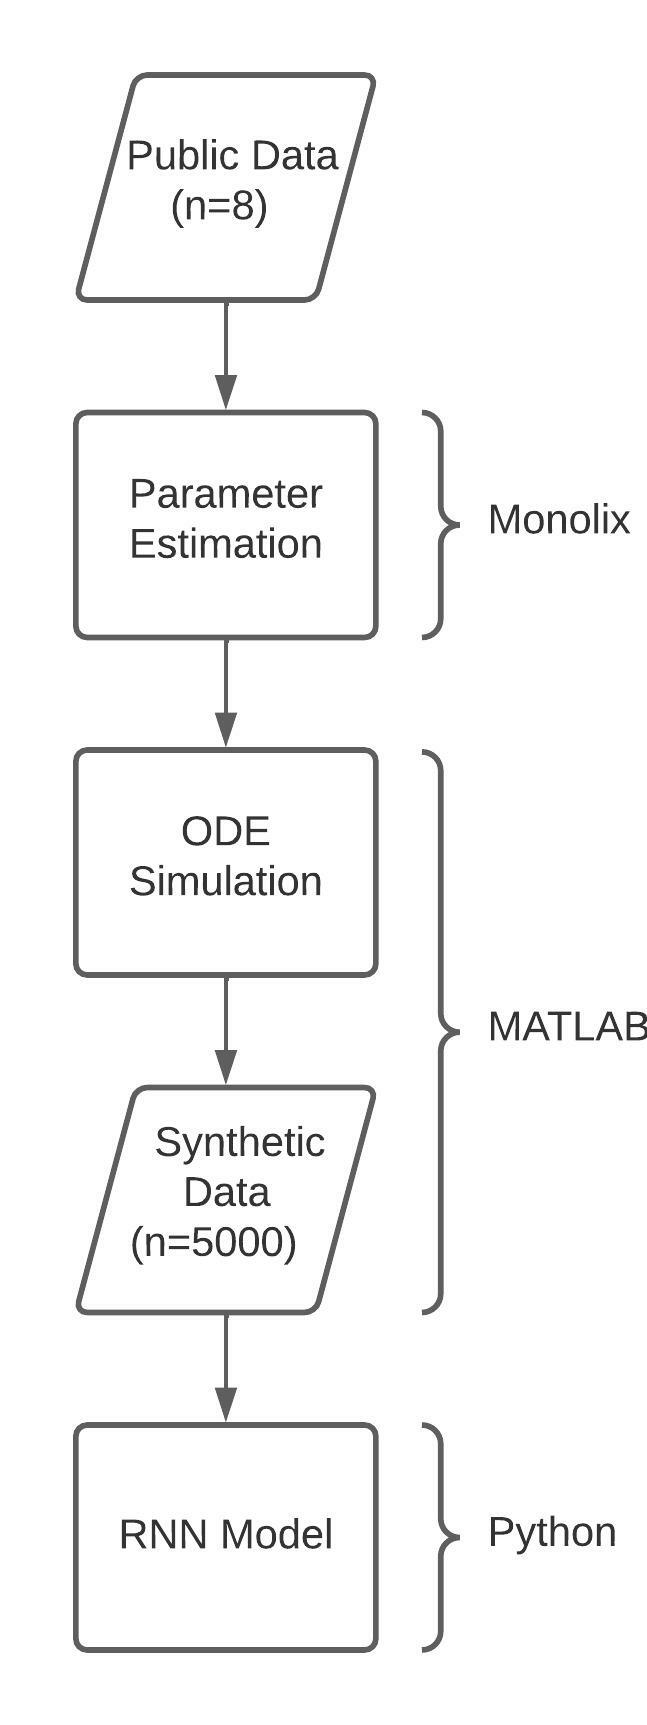
\includegraphics[width=200pt]{Flowchart.jpeg}
\caption{Flowchart of methods.}
\label{fig:flowchart}
\end{figure}

\begin{figure}[ht]
\centering
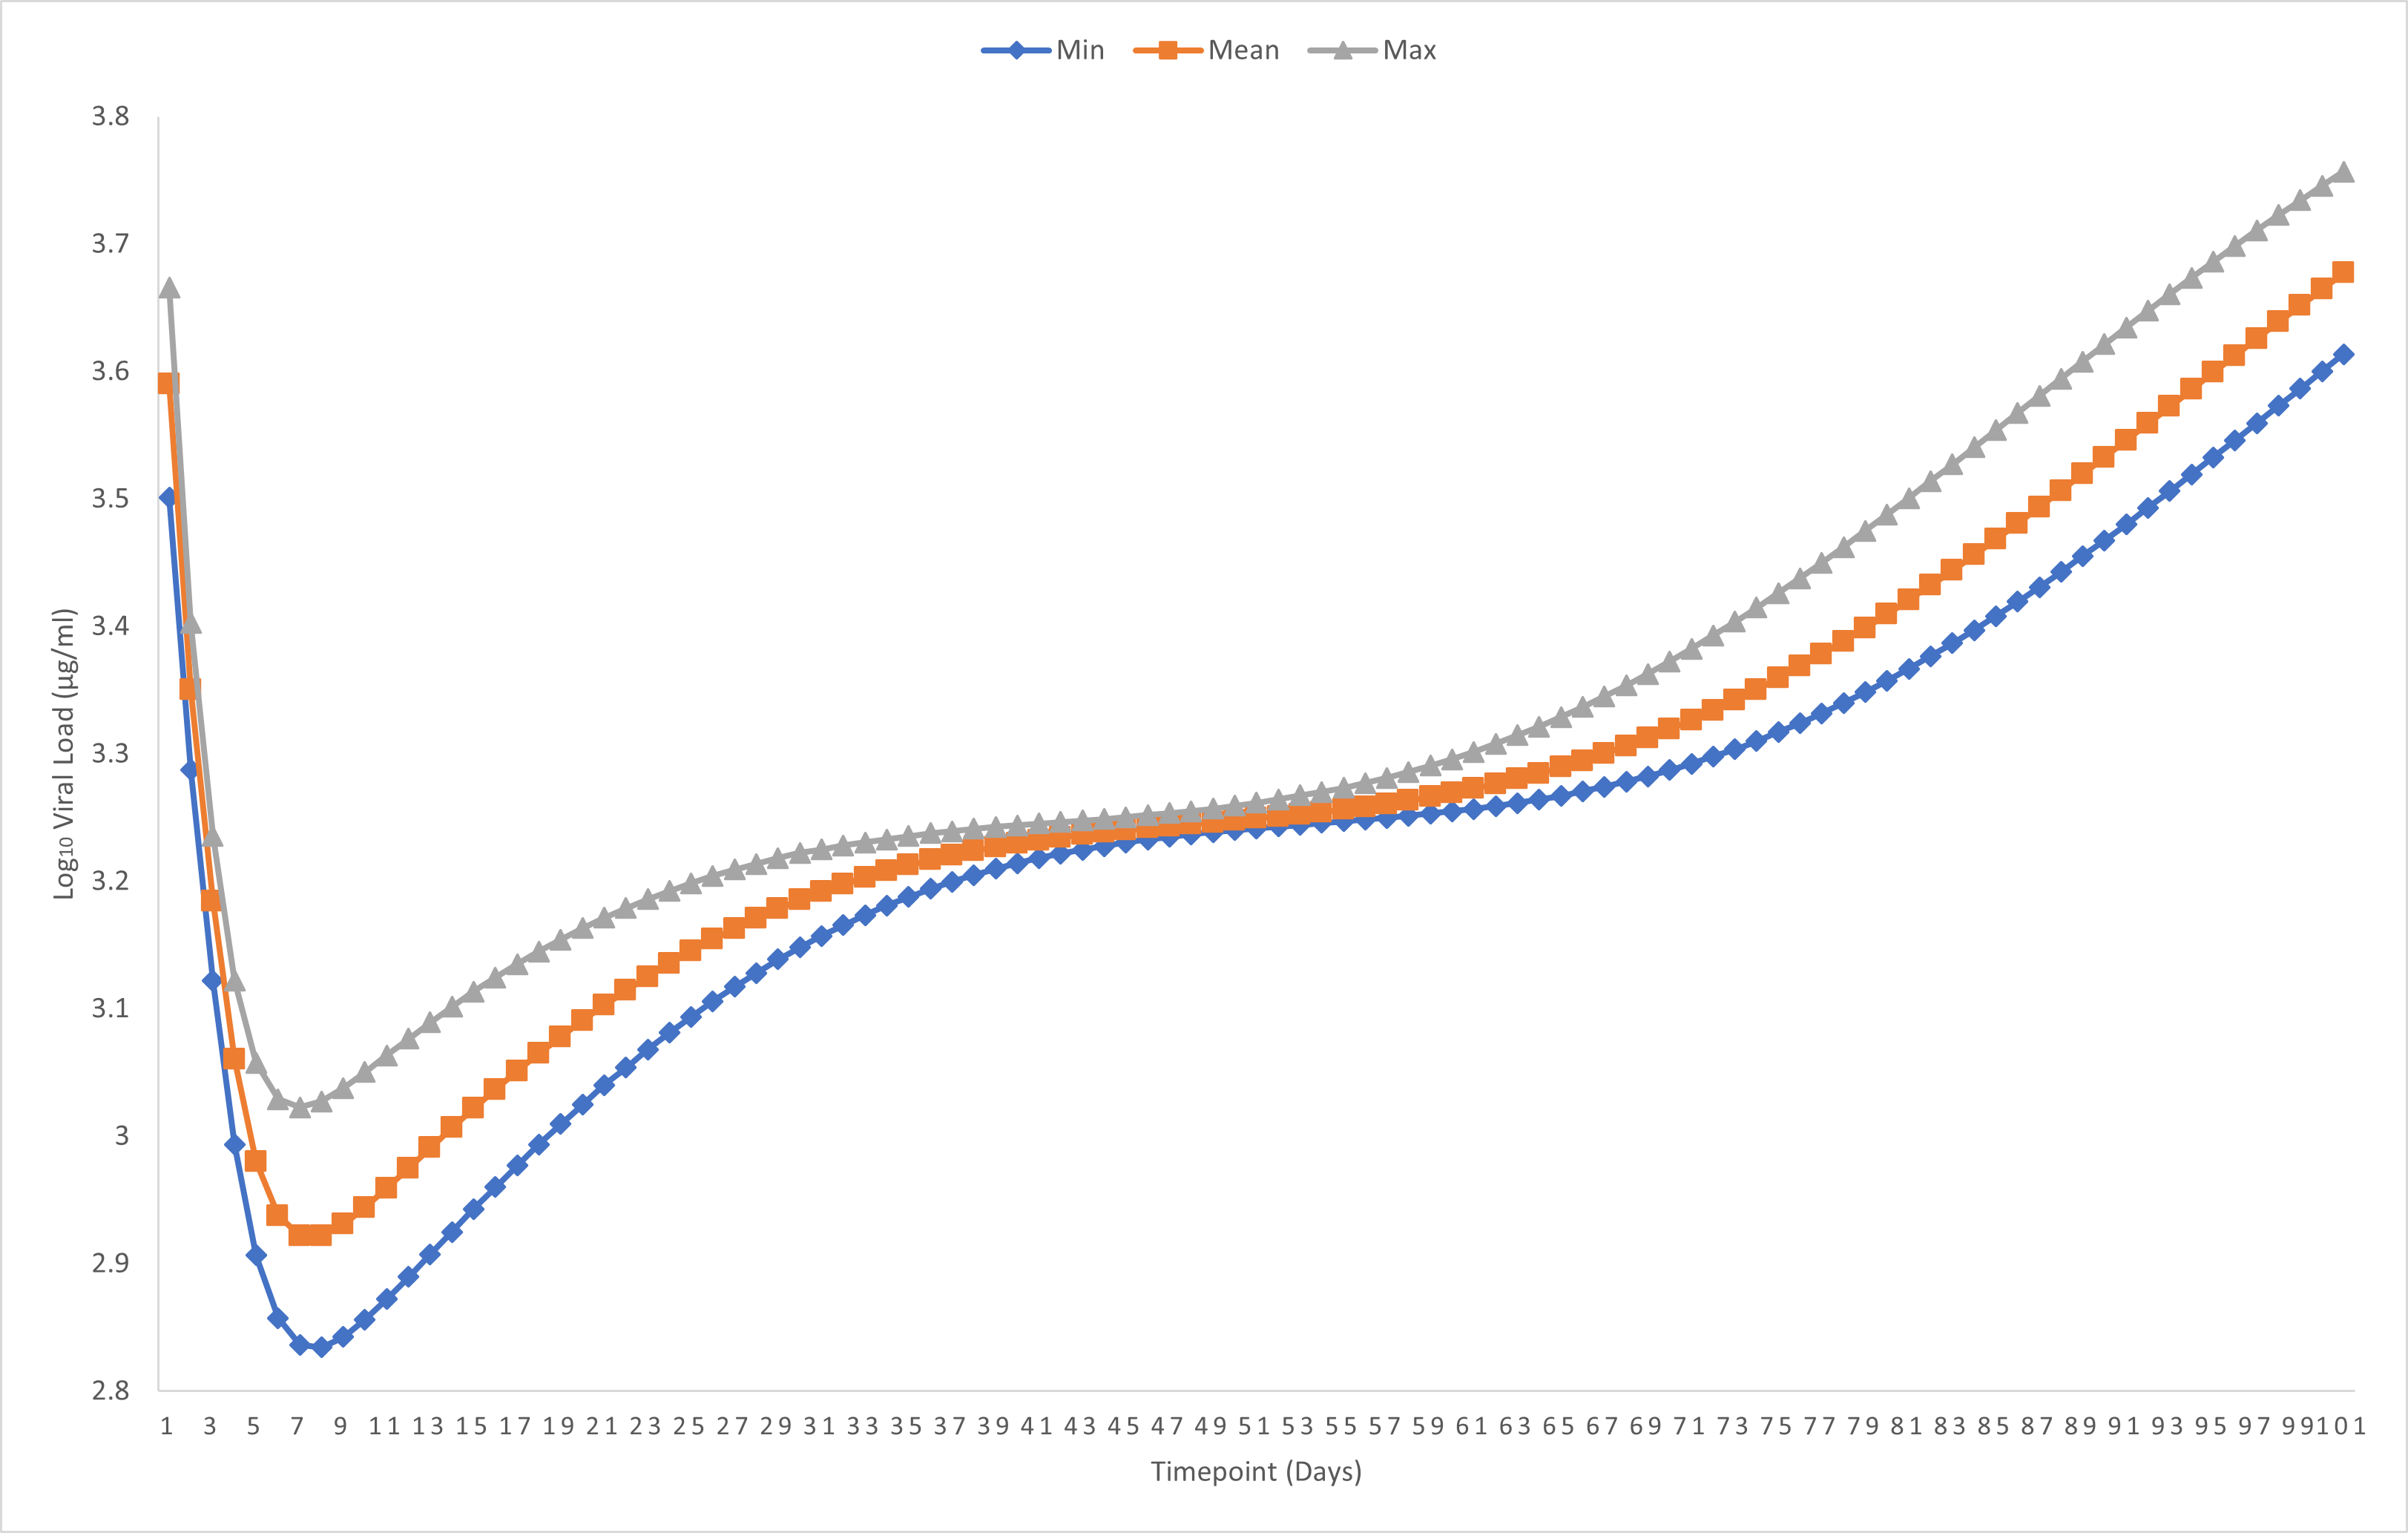
\includegraphics[width= 500pt]{VL.png}
\caption{$VL$ synthetic data.}
\label{fig:VL}
\end{figure}

\begin{figure}[ht]
\centering
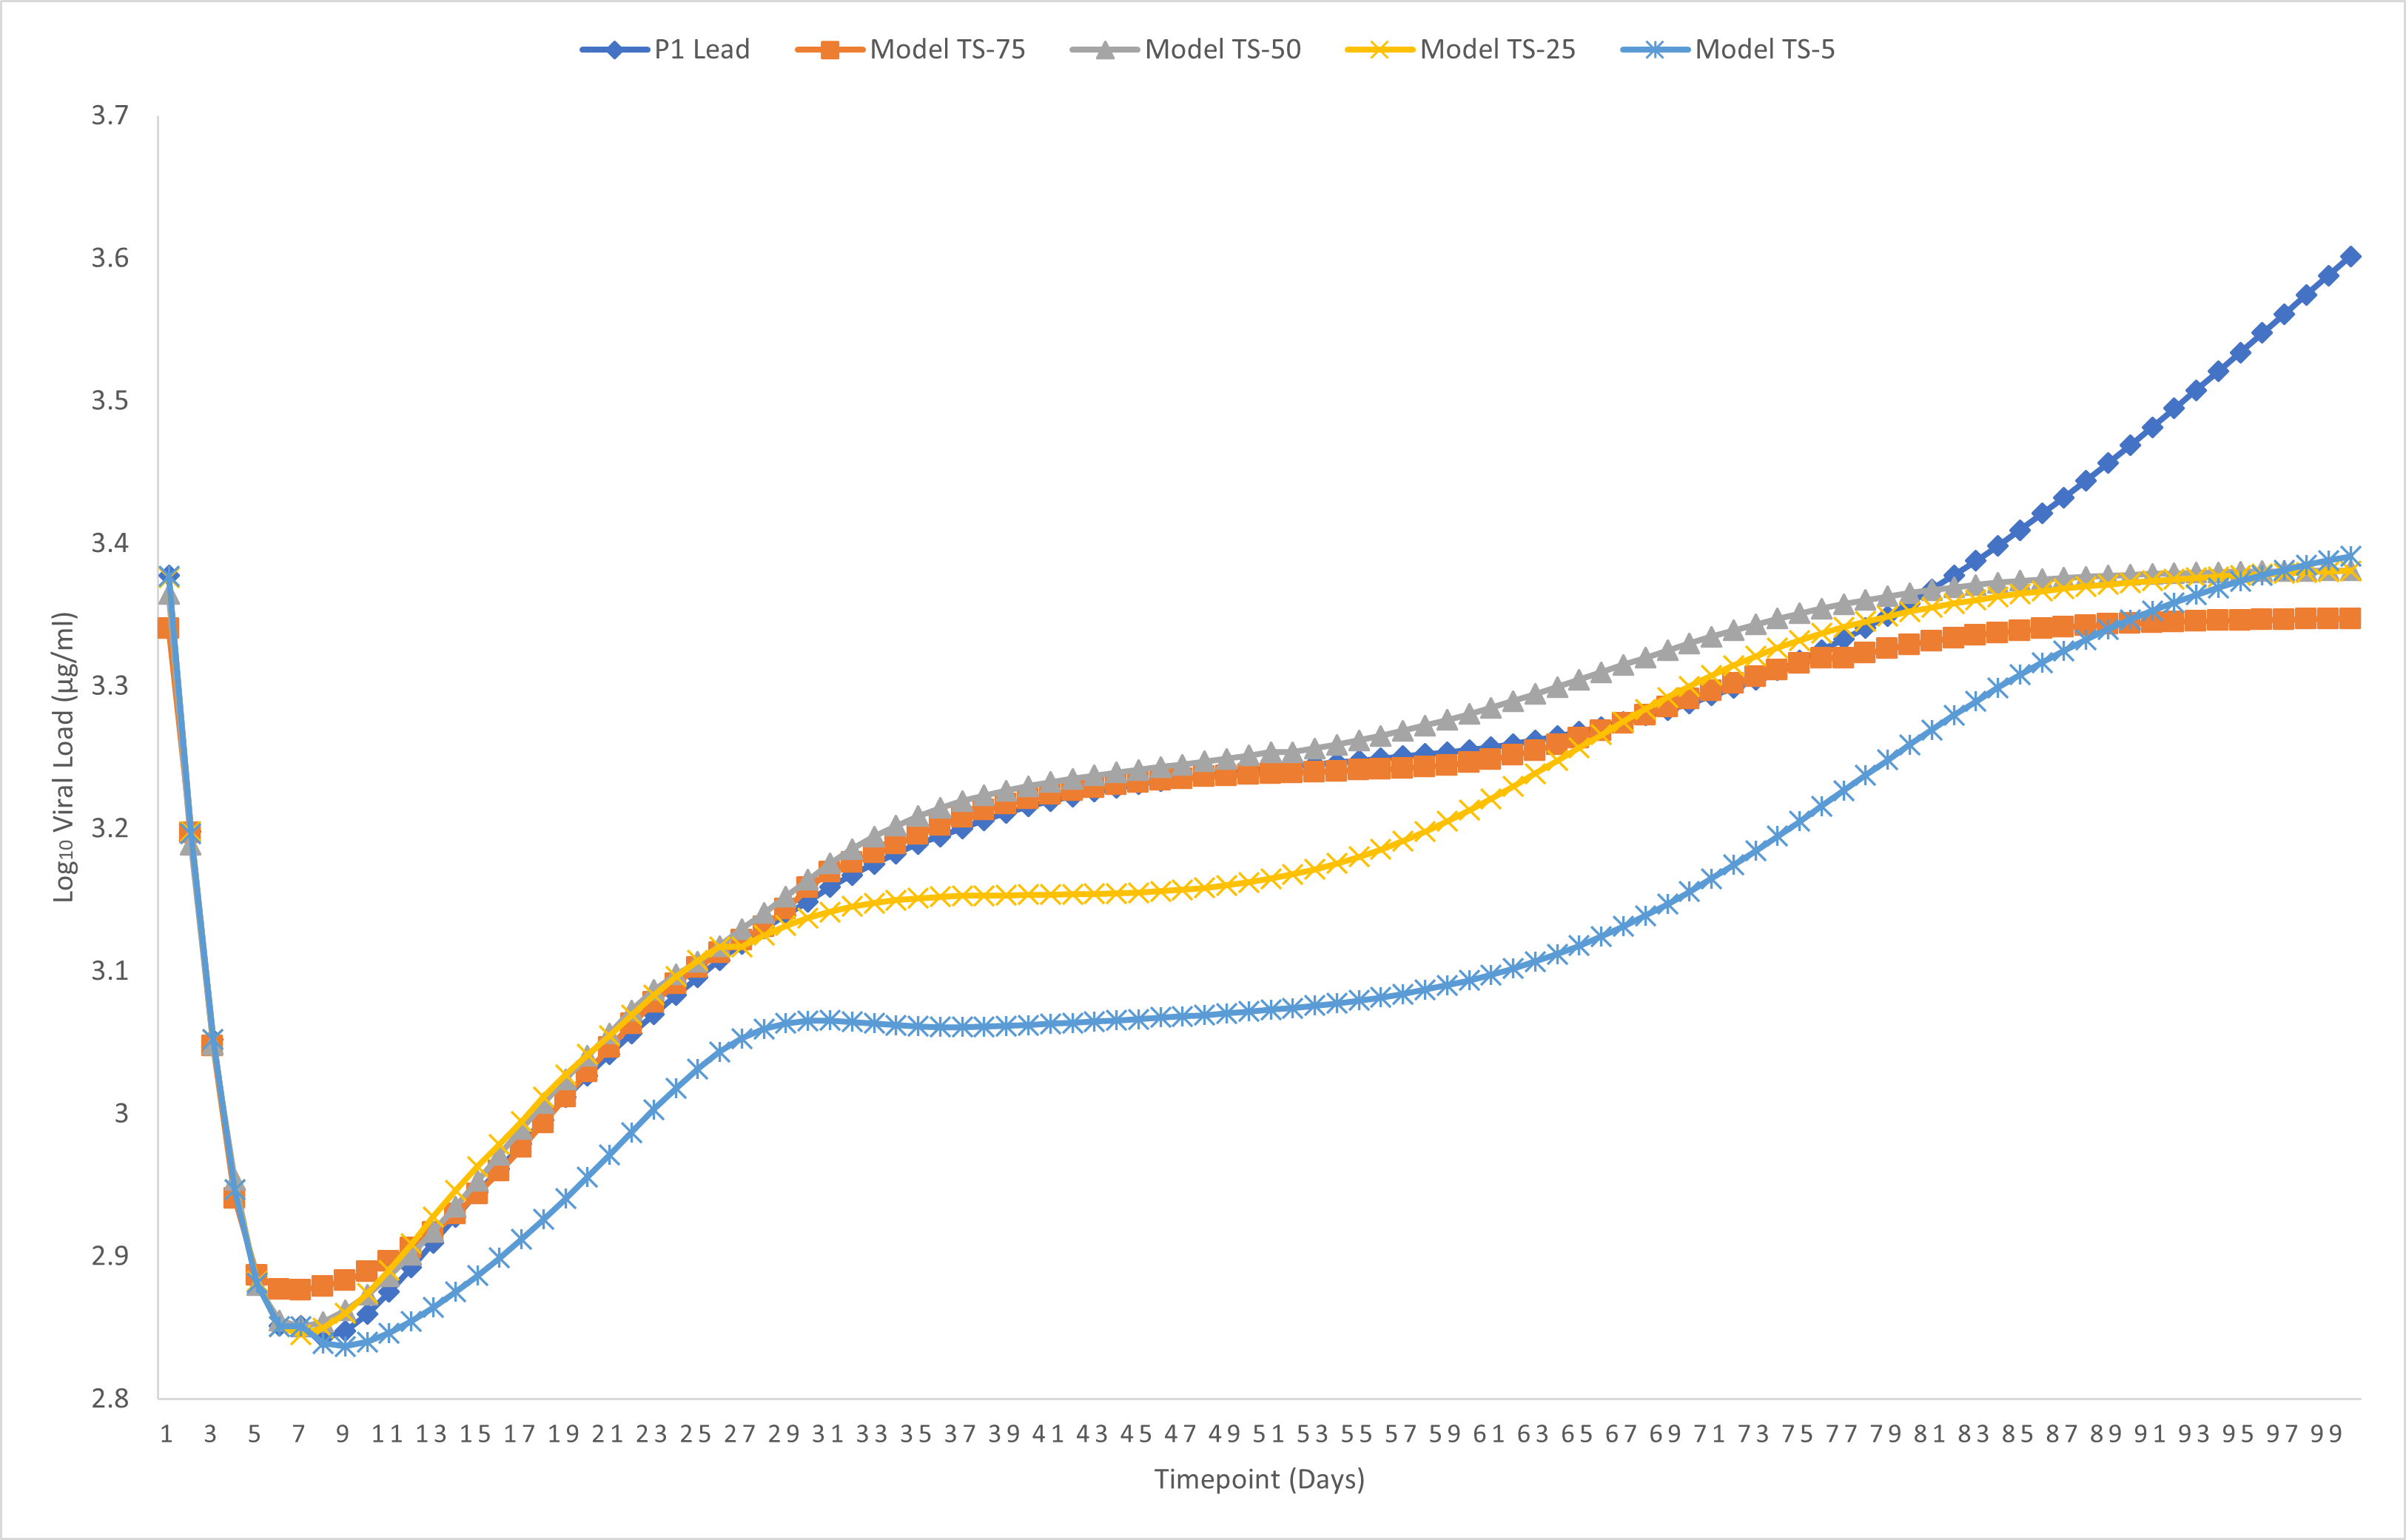
\includegraphics[width= 500pt]{RNN1.png}
\caption{Comparison of LSTM-RNN models with full data and $t=1$ timepoint lead.}
\label{fig:RNN1}
\end{figure}

\begin{figure}[ht]
\centering
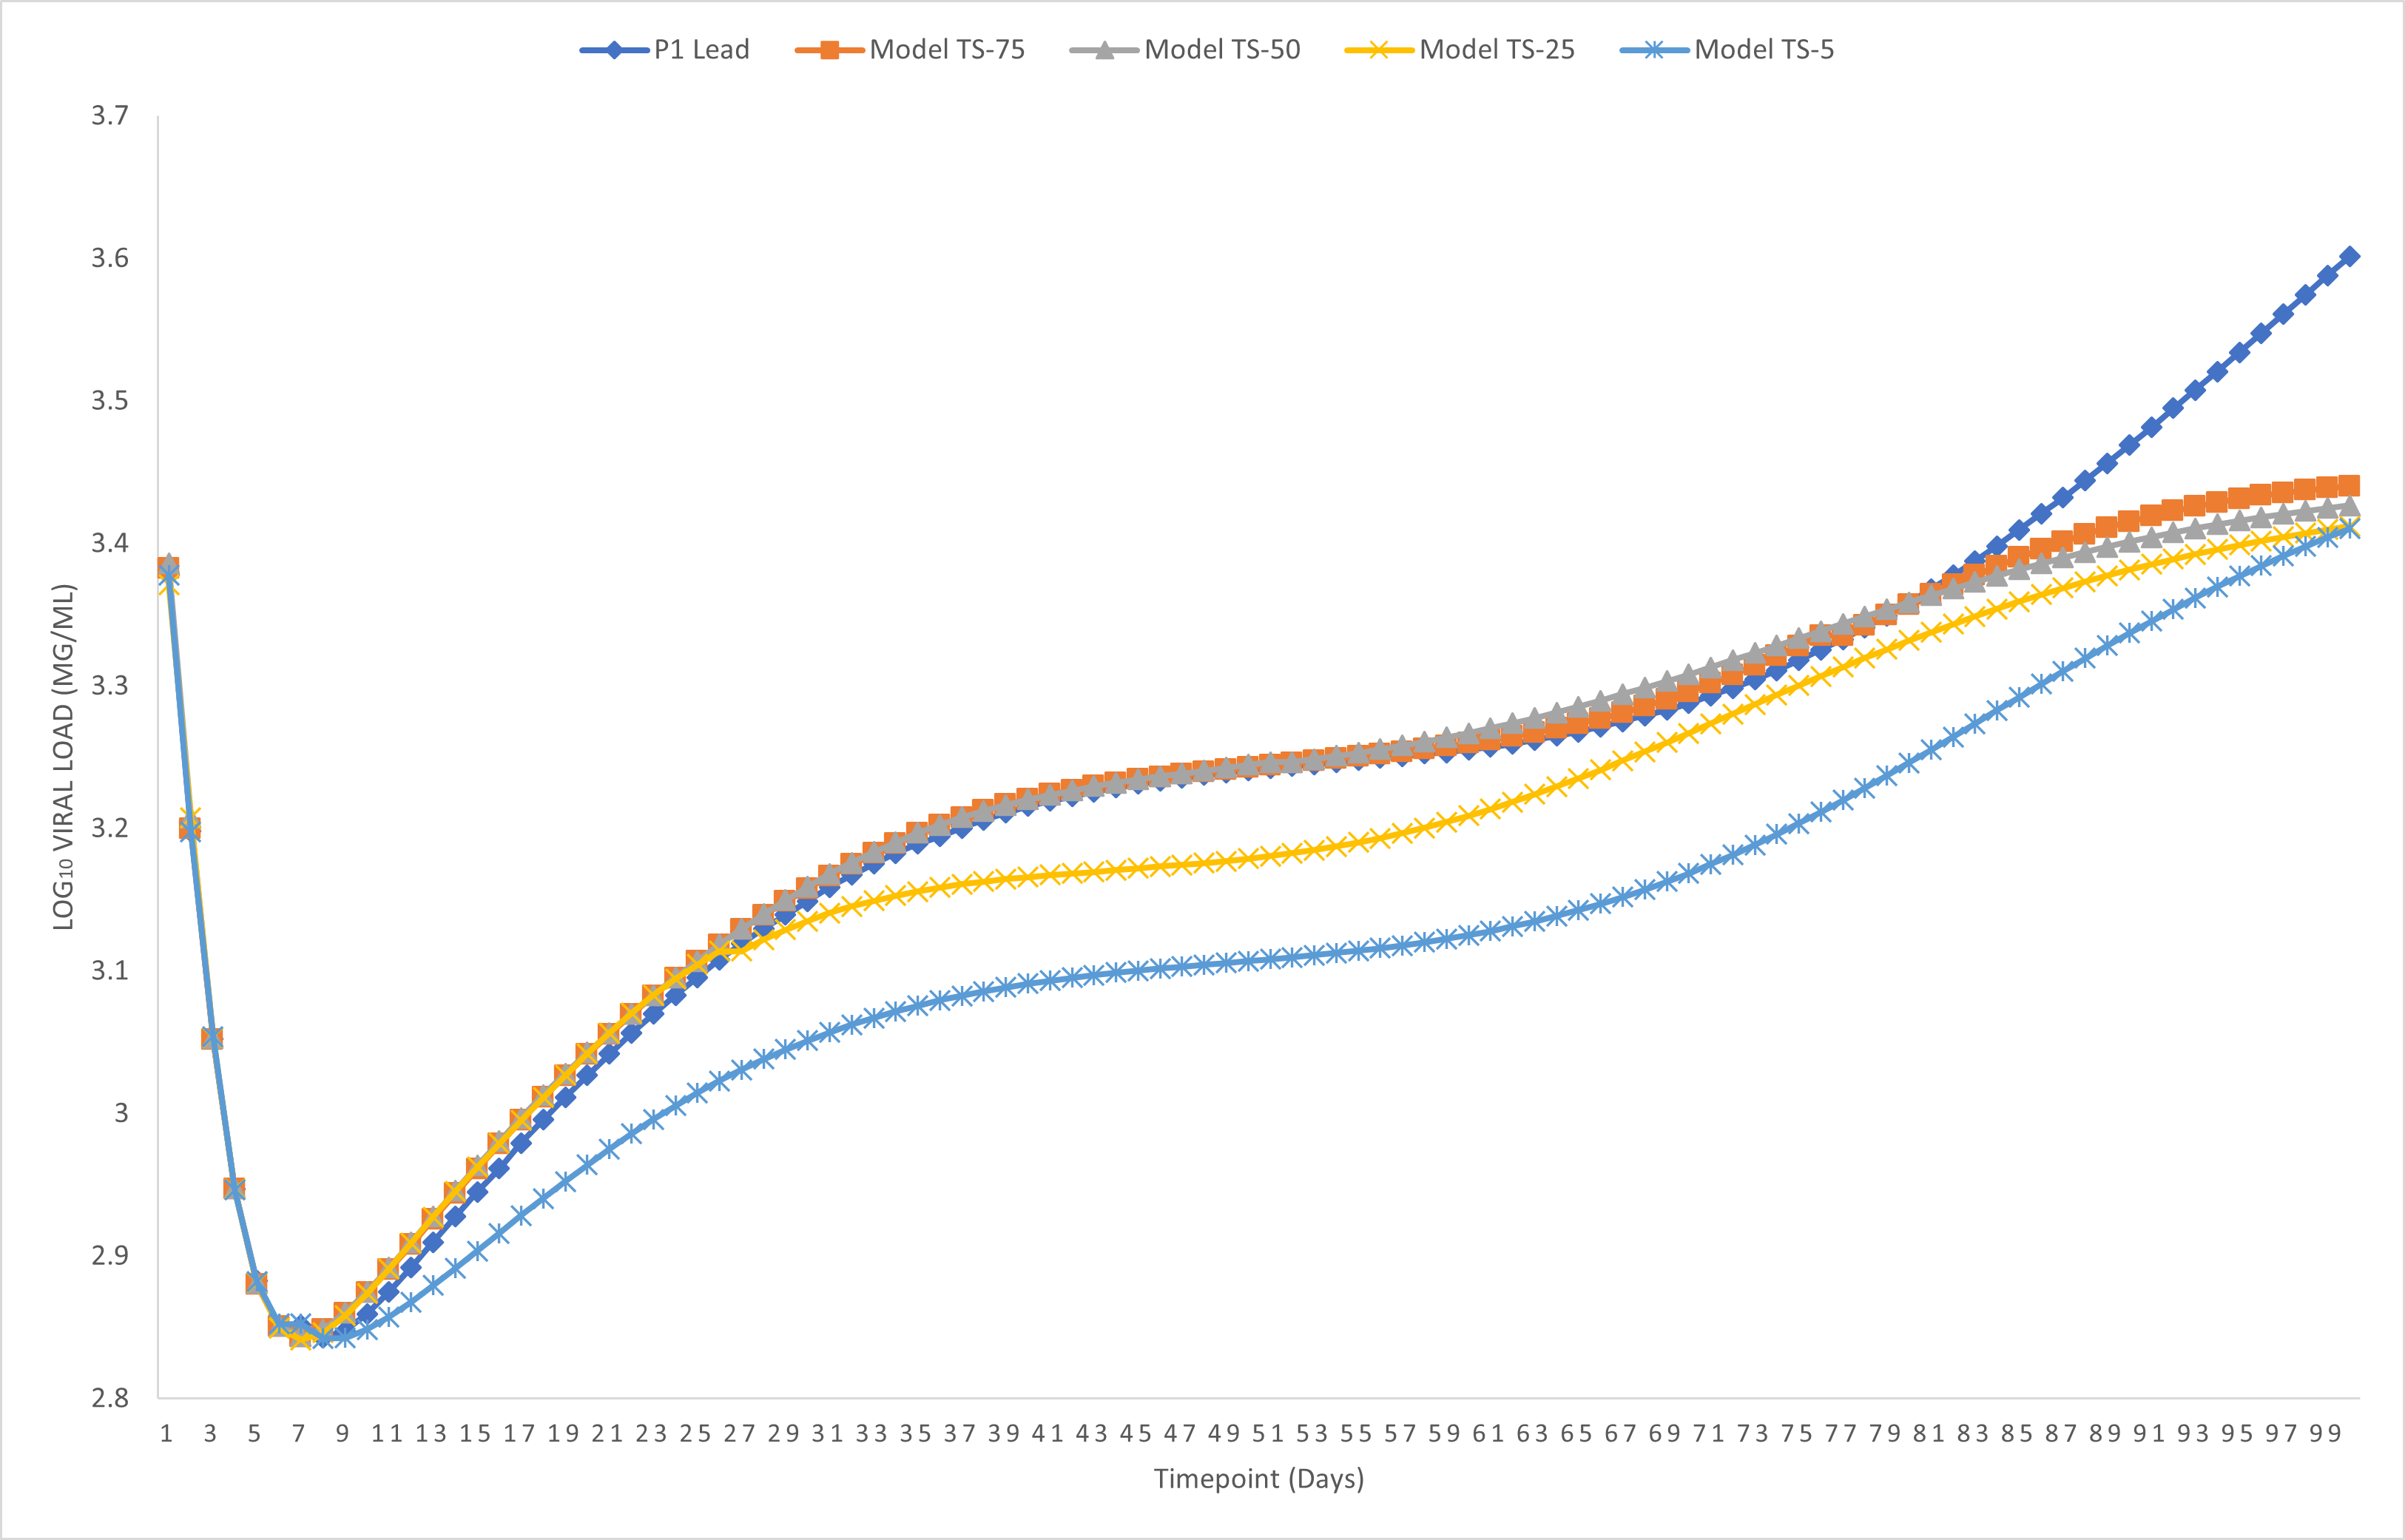
\includegraphics[width= 500pt]{RNN2.png}
\caption{Comparison of LSTM-RNN models with $10\%$ data and $t=1$ timepoint lead.}
\label{fig:RNN2}
\end{figure}

\begin{figure}[ht]
\centering
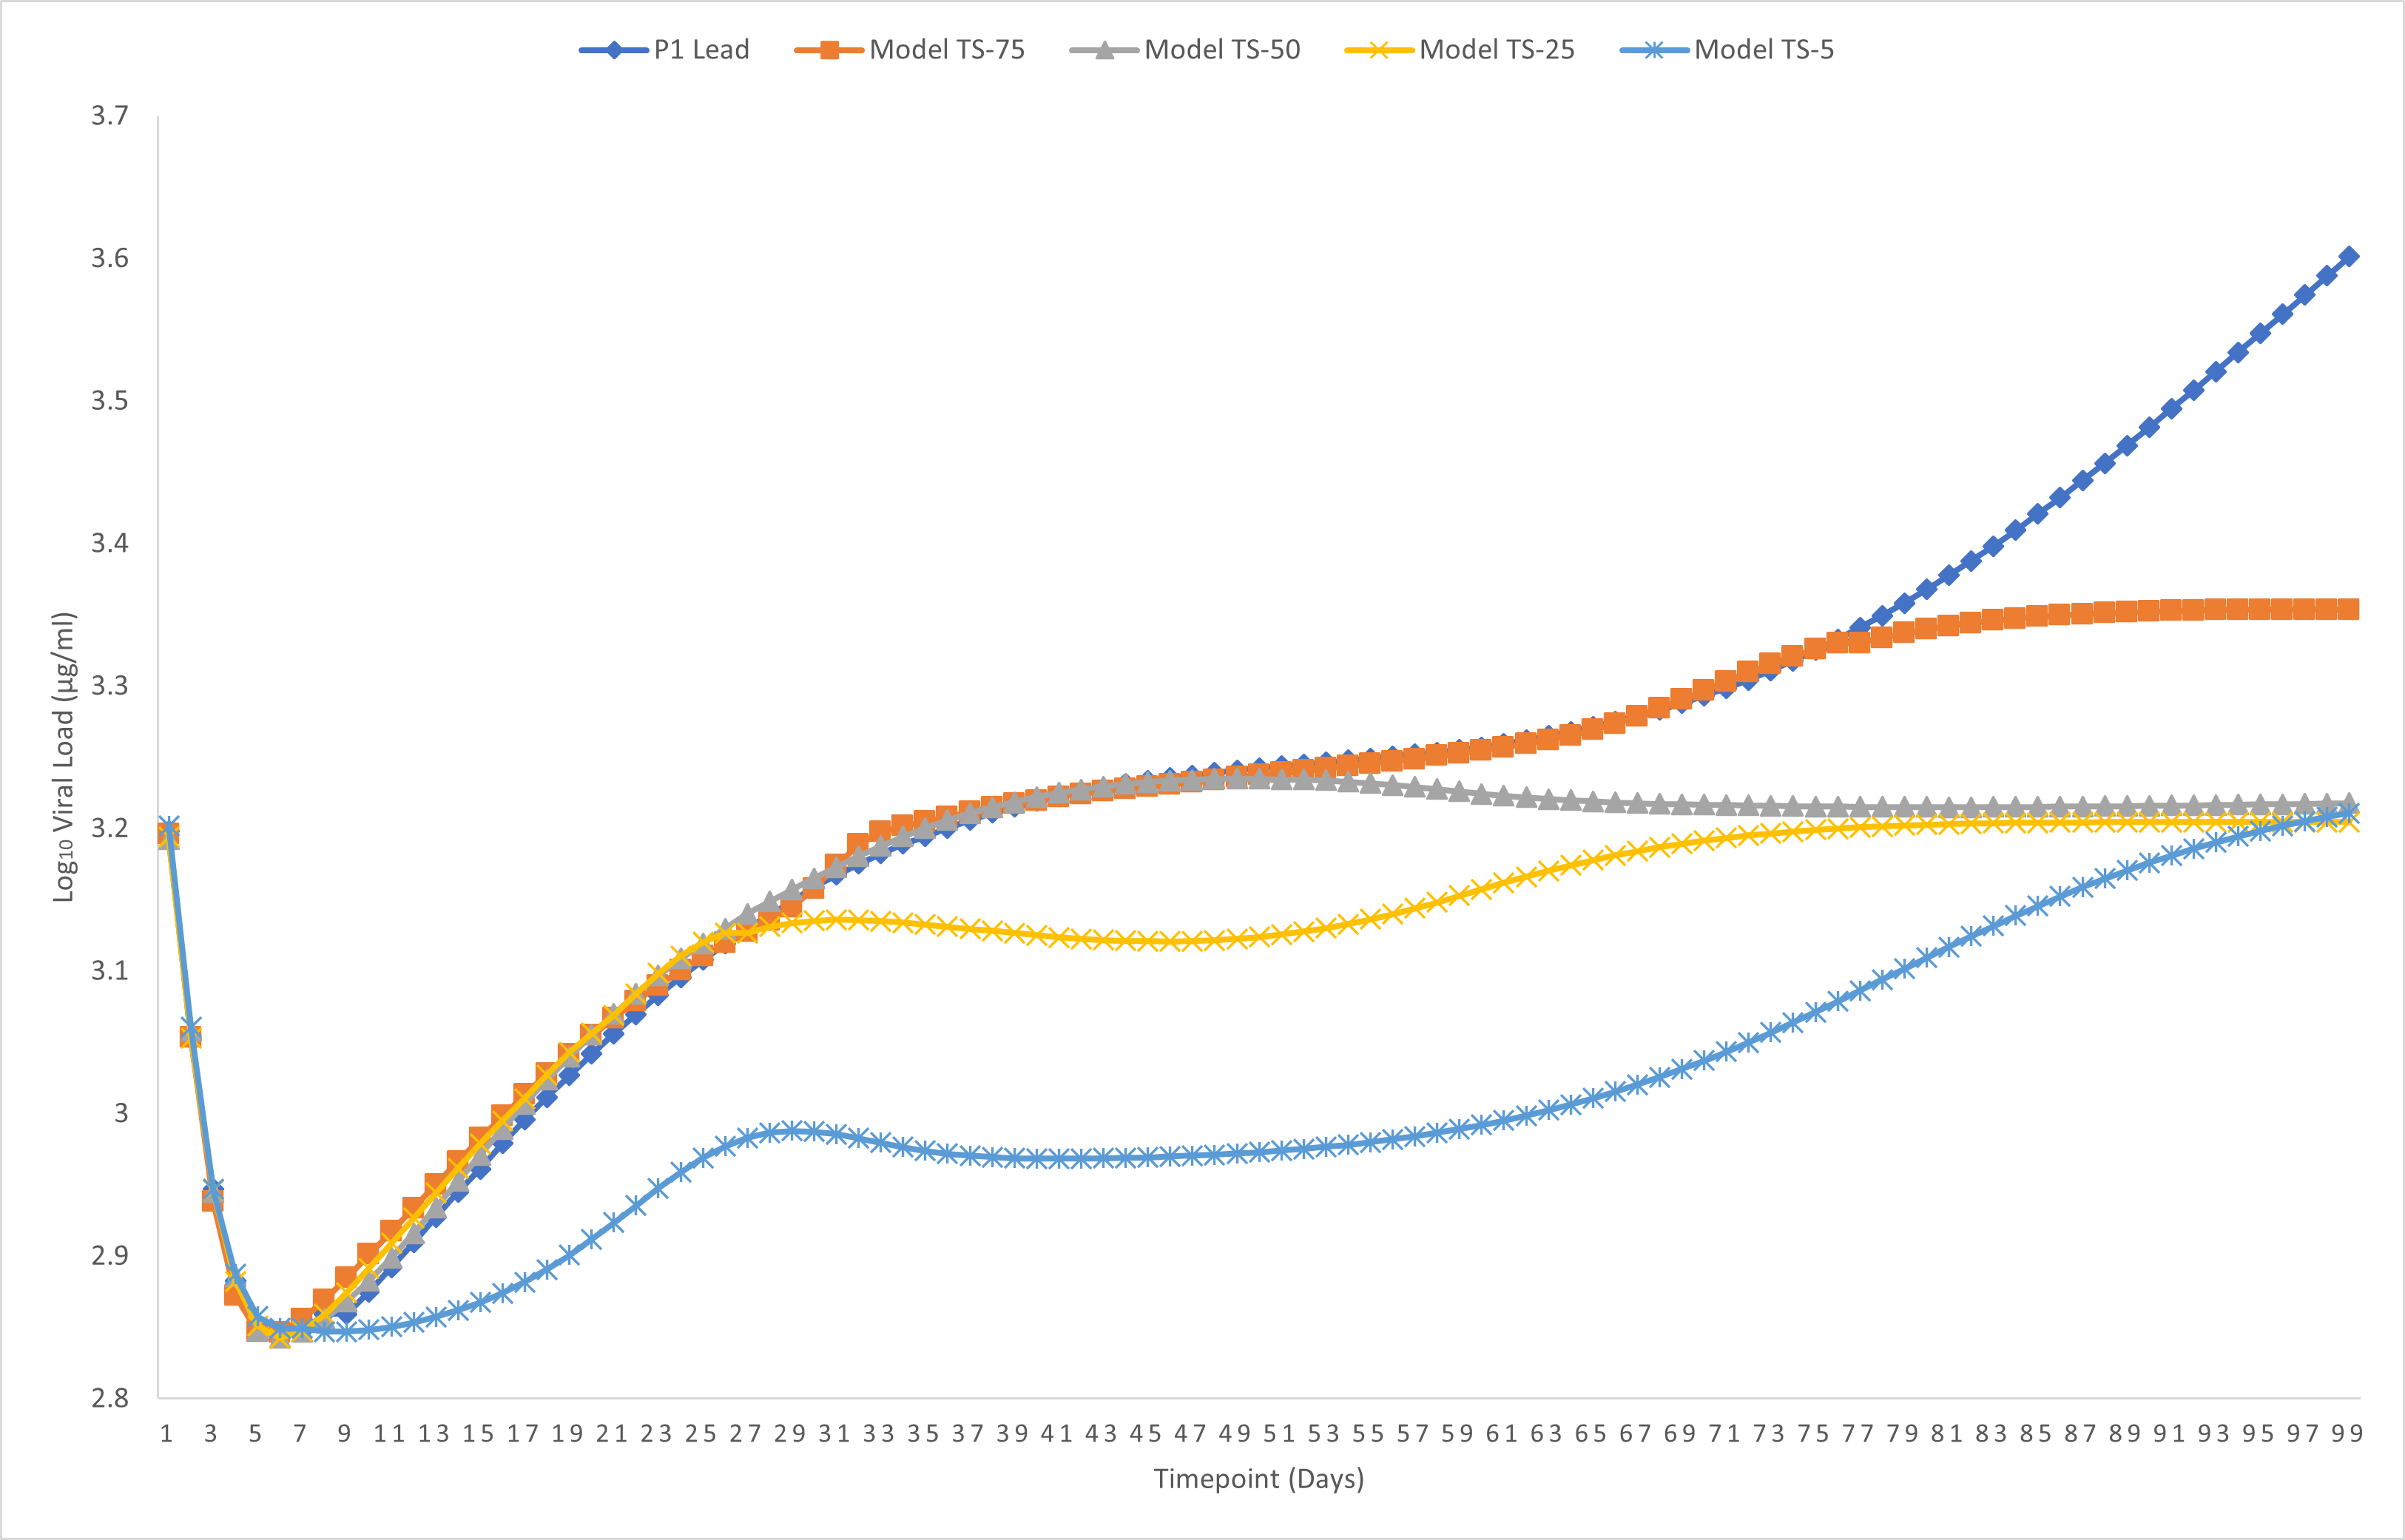
\includegraphics[width= 500pt]{RNN3.png}
\caption{Comparison of LSTM-RNN models with full data and $t=2$ timepoint lead.}
\label{fig:RNN3}
\end{figure}




\begin{table}[ht]
\centering
\begin{tabular}{|l|l|l|l|}
\hline
\textbf{Parameters} & \textbf{Description} & \textbf{Value} & \textbf{Unit} \\
\hline
$d$ & Loss rate of T-cells & $0.01$ & 1/day \\
\hline
$c$ & Clearance rate of free virus & $23$ & 1/ day  \\
\hline
$f$ & Fraction of productively infected cells & $0.05$ & 1/day \\
\hline
$\gamma$ & Clearance rate of immune complexes & $0.5$ & 1/day  \\
\hline
$\omega$ & Effector cell density coefficient & $1.26$ & \\
\hline
$K$ & Carrying capacity of phagocytes & $16$ & copies/ml \\
\hline
$p$ & Production rate of free virus & $3.05$ & 1/day \\
\hline
$k_{Off_s}$ & Disassociation constant of sensitive virus & $13628$ & 1/day \\
\hline
$k_{Off_r}$ & Disassociation constant of resistant virus & $13628$ & 1/day \\
\hline
$k_{On_s}$ & Association constant of sensitive virus & $0.298$ & ml/day \\
\hline
$k_{On_r}$ & Association constant of resistant virus & $2864.47$ & ml/day \\
\hline
$k_{On_i}$ & Association constant of immune complexes & $2.847$ & ml/day \\
\hline
$\delta$ & Death rate of infected cells & $0.0493$ & 1/day \\
\hline
$\beta_s$ & Infectivity of sensitive virus & $2.4433$ & 1/(ml day) \\
\hline
$\beta_r$ & Infectivity of resistant virus & $1.38$ & 1/(ml day) \\
\hline
$\lambda_1$ & Distribution rate to tissues of Ab & $0.5$ & 1/day \\
\hline
$\lambda_2$ & Distribution rate of Ab out of the body & $0.01$ & 1/day \\
\hline
$\lambda$ & Target cell production rate & $1.9806 e6$ & 1/(ml day) \\
\hline
\end{tabular}
\caption{\label{tab:par}Description of model parameters.}
\end{table}

\begin{table}[ht]
\centering
\begin{tabular}{|l|l|l|l|}
\hline
\textbf{Case Number} & \textbf{Model} & \textbf{Train Loss} & \textbf{Test Loss}  \\
\hline
$1$ & $TS-5$ & $7.7e-06$ & $0.44$ \\
\hline
$1$ & $TS-25$ & $1.1e-04$ & $0.45$ \\
\hline
$1$ & $TS-50$ & $9.0e-03$ & $0.48$ \\
\hline
$1$ & $TS-75$ & $9.1e-02$ & $1.34$ \\
\hline
$2$ & $TS-5$ & $1.5e-05$ & $0.34$ \\
\hline
$2$ & $TS-25$ & $4.3e-02$ & $0.35$ \\
\hline
$2$ & $TS-50$ & $2.9e-03$ & $0.29$ \\
\hline
$2$ & $TS-75$ & $2.9e-05$ & $0.46$ \\
\hline
$3$ & $TS-5$ & $4.1e-02$ & $3.2$ \\
\hline
$3$ & $TS-25$ & $2.0e-03$ & $3.3$ \\
\hline
$3$ & $TS-50$ & $1.8e-02$ & $2.4$ \\
\hline
$3$ & $TS-75$ & $5.7e-02$ & $1.0$ \\
\hline
\end{tabular}
\caption{\label{tab:eval}Evaluation of LSTM-RNN Models at Epoch $400$.}
\end{table}

\end{document}